\section{Counterfactual Evaluation and Learning to Rank}
\begin{itemize}
	\item The term \textit{counterfactual} relates to \textit{off-policy} learning in RL
	\item Thus, we try to evaluate an offline task by using online data obtained by another policy to estimate the performance of the new policy in a online setting
\end{itemize}
\subsection{Counterfactual Evaluation}
\begin{itemize}
	\item In general, a user interactive system can be formalized as follows (see Figure~\ref{img:counterfactual_user_interactive_system}):
	\begin{itemize}
		\item $x$: Feature vector describing the user and context (i.e. query)
		\item $y$: Result the system returns based on its policy ($y=\pi(x)$)
		\item $\delta$: Feedback signal from the actions a user took. The function encodes the metric (user utility function) and is defined as $\delta: X\times Y\to \mathbb{R}$
		\item $\pi$: Policy describing the ranking system which takes $x$ as input and maps it to output $y$: $\pi:X\to Y$
	\end{itemize}
	\begin{figure}[ht]
		\centering
		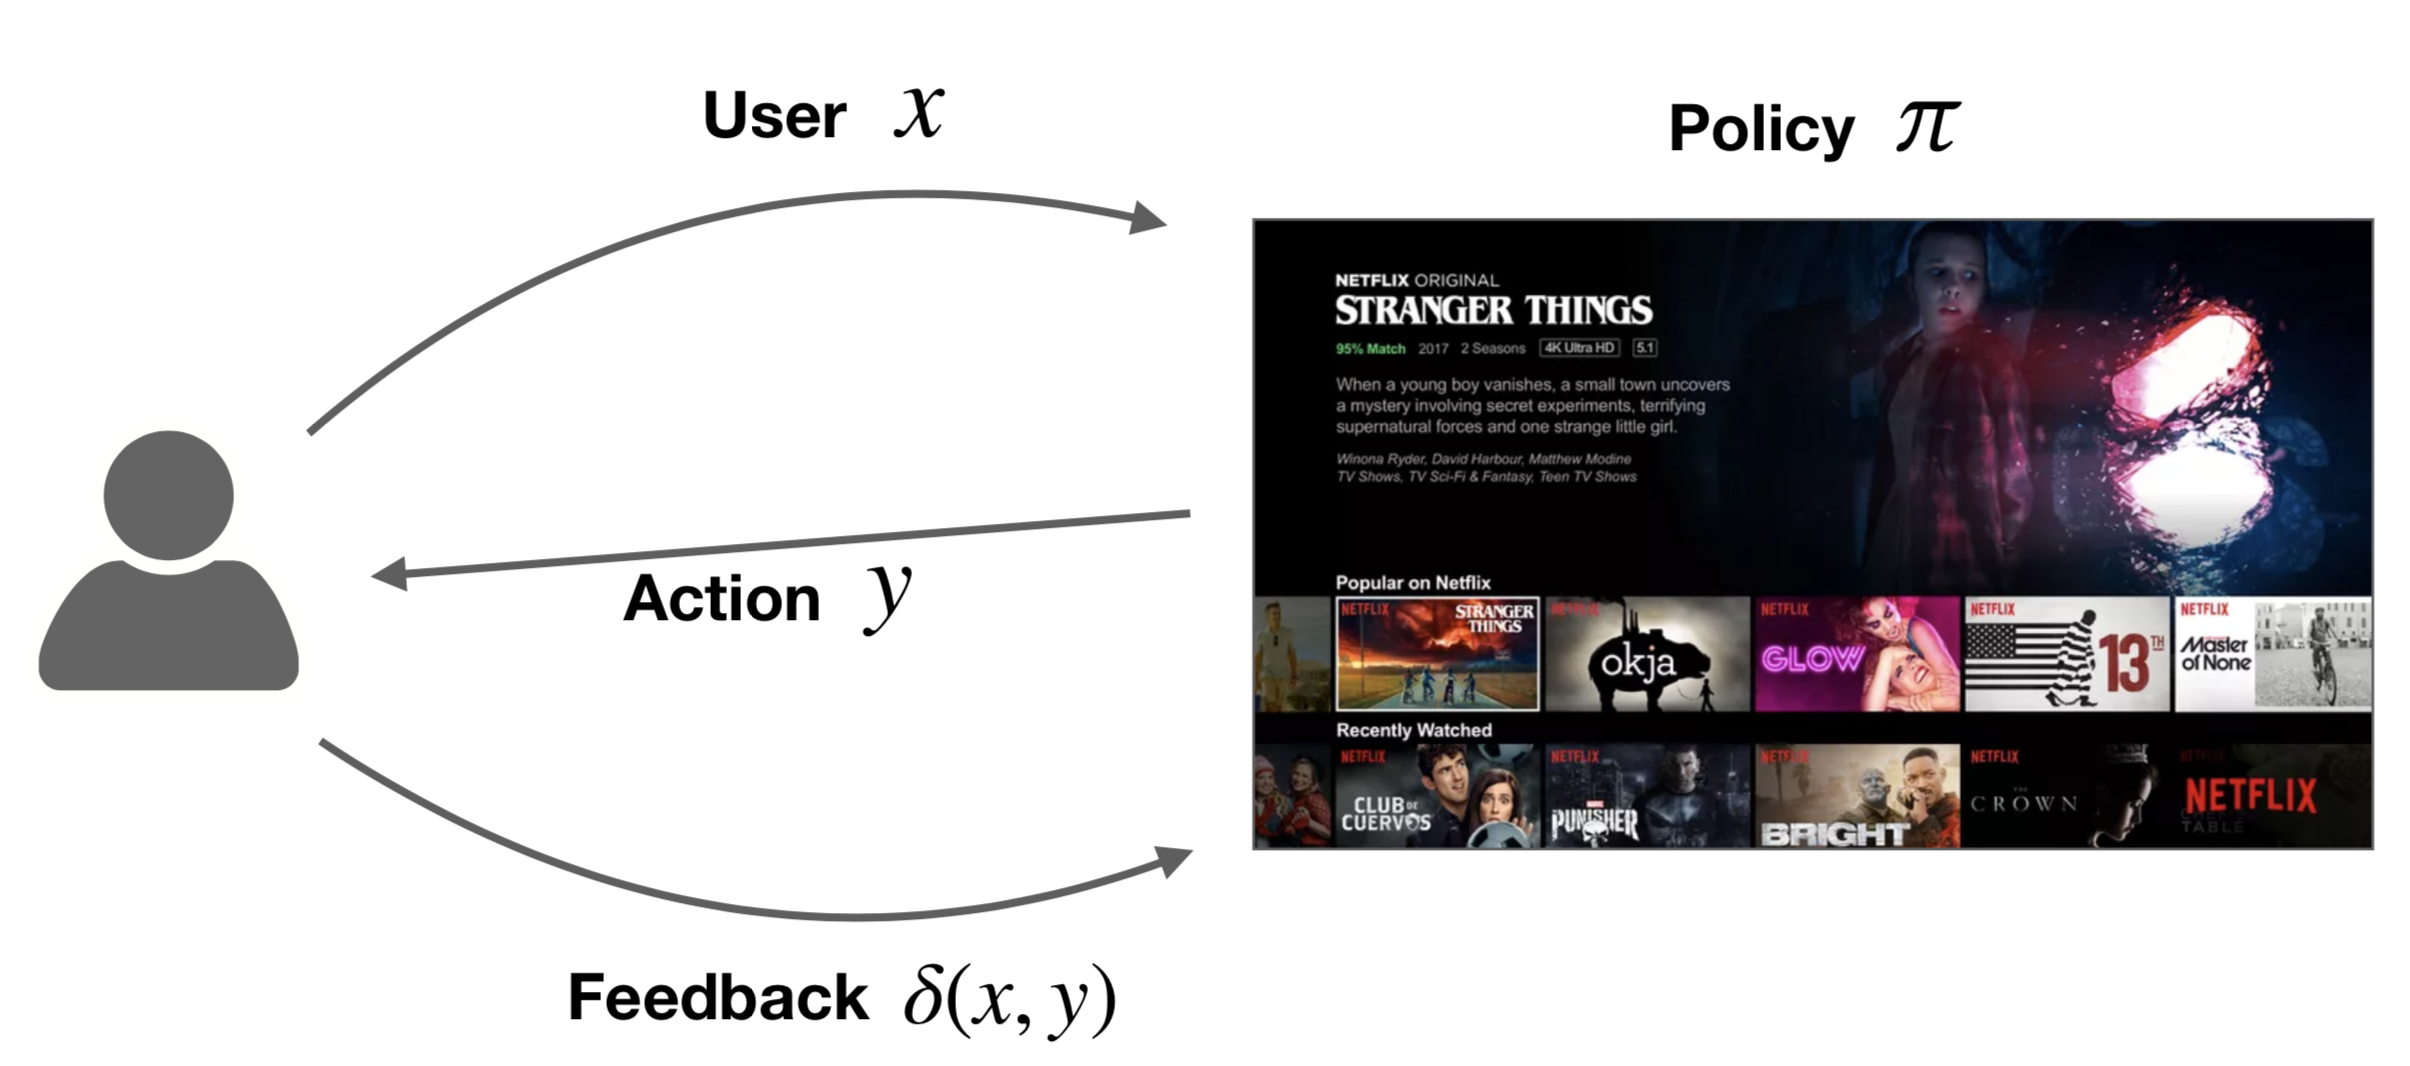
\includegraphics[width=0.5\textwidth]{figures/counterfactual_user_interactive_system.png}
		\caption{Visualization fo a user interactive system}
		\label{img:counterfactual_user_interactive_system}
	\end{figure}
	\item \textit{Counterfactual evaluation}: perform offline evaluation of online metrics given online data from another system $\pi_{\text{production}}$. Thus, we try to estimate performance of $\pi_{\text{new}}$ with interaction data obtained with $\pi_{\text{production}}$.
	\item The interactions data/log is structured as $D=\left\{\left(x_1, y_1, \delta_1\right),...,\left(x_n, y_n, \delta_n\right)\right\}$
	\begin{itemize}
		\item The actions $y_i$ were selected by $\pi_{\text{production}}:X\to Y$
		\item Note that we only have partial information feedback, and no complete supervision. Only for the chosen action, we know the feedback signal/user utility. Thus, the "correct"/optimal action is unknown (also called "bandit feedback" as it was sampled from only one arm)
	\end{itemize}
	\item We want to estimate $\mathbb{E}_{y\sim \pi_{\text{new}}}\left[\delta(x,y)\right]$ given $D$ from $\pi_{\text{production}}$. For this, there are two approaches: \textit{model the rewards} and \textit{inverse propensity scoring}.
\end{itemize}
\subsubsection{Model the rewards}
\begin{itemize}
	\item The intuition behind \textit{model the rewards} is to learn the reward function $\delta:X\times Y\to \mathbb{R}$ from $D\sim \pi_{\text{production}}$ directly
	\item The task can be reduced to a regression problem: $$\delta_w = \arg\min_{\delta_w} \sum\limits_{i=1}^{N} \mathcal{L}\left(\delta_w\left(x_i, y_i\right), \delta_i \right)$$
	where $\mathcal{L}$ is a loss function like MSE.
	\item Once $\delta_w$ is learned, we can estimate our goal by $\mathbb{E}_{y\sim \pi_{\text{new}}}\left[\delta(x,y)\right] = \frac{1}{n} \sum\limits_{i=1}^{N} \delta_w \left(x_i, \pi_{\text{new}}(x_i)\right)$
	\item However, learning $\delta_w$ is in general very difficult, as:
	\begin{itemize}
		\item Input space $X\times Y$ is very high-dimensional
		\item Rewards are highly non-linear and noisy
		\item Data is strongly biased to the actions that $\pi_{\text{production}}$ prefers
	\end{itemize}
\end{itemize}
\subsubsection{Inverse Propensity Scoring}
\begin{itemize}
	\item Instead of learning $\delta_w$, is it possible to directly estimate the value of the new policy $\pi_{\text{new}}$?
	\item Answer: only under the condition that the policy $\pi_{\text{production}}$ is stochastic: $y\sim \pi(y|x)$. The probability $p$ to choose the action $y$ is also called \textit{propensity}. Note that $p>0$ must hold for all possible actions as we otherwise have no chance to discover/obtain feedback for all actions
	\item For unbiased counterfactual evaluation, we need data samples with the propensity $p_i$ from policy $\pi_{\text{production}}$ describing the probability of selecting $y_i$ for given input $x_i$: $\left(x_i, y_i, \delta_i, p_i\right)$
	\item Use importance sampling to make distributions $\pi_{\text{production}}$ and $\pi_{\text{new}}$ comparable. This leads to the \textbf{IPS-estimator}:
	$$\frac{1}{n}\sum\limits_{i=1}^{N} \delta_i \frac{\pi_{\text{new}}(y_i|x_i)}{p_i}$$
\end{itemize}
\subsubsection{Proof of Unbiasedness}
\begin{itemize}
	\item We want to proof that in expectation, the IPS estimator will lead to the correct value: $$\mathbb{E}_{y\sim \pi_{\text{production}}}\left[\frac{1}{n}\sum\limits_{i=1}^{N} \delta_i \frac{\pi_{\text{new}}(y_i|x_i)}{p_i}\right] = \mathbb{E}_{y\sim \pi_{\text{new}}}\left[\delta(x,y)\right]$$
	\item First, we can put the sum outside the expectation:
	$$\mathbb{E}_{y\sim \pi_{\text{production}}}\left[\frac{1}{n}\sum\limits_{i=1}^{N} \delta_i \frac{\pi_{\text{new}}(y_i|x_i)}{p_i}\right] = \frac{1}{n}\sum\limits_{i=1}^{N} \mathbb{E}_{y\sim \pi_{\text{production}}}\left[\delta_i \frac{\pi_{\text{new}}(y_i|x_i)}{p_i}\right]$$
	\item Next, we replace the expectation by a sum over actions weighted by their corresponding probabilities:
	$$\frac{1}{n}\sum\limits_{i=1}^{N} \mathbb{E}_{y\sim \pi_{\text{production}}}\left[\delta_i \frac{\pi_{\text{new}}(y_i|x_i)}{p_i}\right] = \frac{1}{n}\sum\limits_{i=1}^{N} \sum\limits_{y_i\in Y}\left[\pi_{\text{production}}(y_i|x_i)\delta_i \frac{\pi_{\text{new}}(y_i|x_i)}{p_i}\right]$$
	\item As $p_i$ is defined as $\pi_{\text{production}}(y_i|x_i)$, we can reduce the equation to:
	$$\frac{1}{n}\sum\limits_{i=1}^{N} \sum\limits_{y_i\in Y}\left[\pi_{\text{production}}(y_i|x_i)\delta_i \frac{\pi_{\text{new}}(y_i|x_i)}{p_i}\right] = \frac{1}{n}\sum\limits_{i=1}^{N} \sum\limits_{y_i\in Y}\left[\delta_i \pi_{\text{new}}(y_i|x_i)\right]$$
	\item Finally, we apply rules based on the definition of expectation:
	$$\frac{1}{n}\sum\limits_{i=1}^{N} \sum\limits_{y_i\in Y}\left[\delta_i \pi_{\text{new}}(y_i|x_i)\right] = \frac{1}{n}\sum\limits_{i=1}^{N} \mathbb{E}_{y_i\sim \pi_{\text{new}}}\left[\delta(x_i,y_i)\right] = \mathbb{E}_{y\sim \pi_{\text{new}}}\left[\delta(x,y)\right]$$
	\item Note that the IPS estimator has a high variance which scales with $p_i^2$. Thus, if we have a very low probability for some actions, this can introduce a high error $\implies$ many samples needed to approximate target accurately. There are different approaches to reduce the variance
\end{itemize}
\subsection{Counterfactual Learning to Rank}
\begin{itemize}
	\item Learning to Rank: \textit{offline} - train on labeled data, \textit{online} - learn from user interactions, \textit{counterfactual} - learn offline from online retrieved data obtained by another policy/ranker
	\item The goal of counterfactual LTR is to learn a new ranker $\pi_{\text{new}}$ from the interaction data with $\pi_{\text{production}}$
	\begin{itemize}
		\item The data is specified by $D=\left\{(x_1,y_1,\delta_1),...,(x_N,y_N,\delta_N)\right\}$ where $\delta_i$ indicates which document was clicked (we assume that only one document was clicked)
		\item $y_i$ is the ranking selected by $\pi_{\text{production}}:X\to Y$
	\end{itemize}
	\item Naive approach: assume click indicates relevance and learn as if it would be a supervised dataset: $$\pi_{\text{new}} = \arg\min_{\pi} \sum\limits_{i=1}^{N} \text{rank}\left(\pi(x_i),y_i,\delta_i\right)$$
	The objective function is to reduce the rank of the relevant document given the new ranking of $\pi_{\text{new}}$ and the previous ranking by $y_i$. Can be solved by pairwise LTR objective.
	\item However, data obtained by online Learning to Rank is commonly noisy and biased
	\item We can take these biases into account by using the inverse propensity scores:
	$$\pi_{\text{new}} = \arg\min_{\pi} \sum\limits_{i=1}^{N} \frac{\text{rank}\left(\pi(x_i),y_i,\delta_i\right)}{p(\textit{observing }\delta_i)}$$
	This formula can be motivated from a probabilistic click model perspective:
	$$p(\textit{click}) = p(\textit{observation})\times p(\textit{relevant}) \implies p(\textit{relevant}) = \frac{p(\textit{click})}{p(\textit{observation})}$$
	Left side is what we want to get, and on the right side it is specified what we actually optimize.
\end{itemize}
\subsubsection{Propensity estimation}
\begin{itemize}
	\item However, the question remains how we calculate $p(\textit{observing }\delta_i)$. We can either approximate it by using click models, or by performing a randomization test
	\item \textit{RandTopN}
	\begin{itemize}
		\item Randomly shuffle the top $N$ documents
		\item Measure clicks people have performed on the data (online experiment)
		\item Aggregate clicks for infinite samples
		\item Infer $\hat{p} \propto p(\textit{observing} \delta_i)$
	\end{itemize} 
	\item \textit{RandPair}
	\begin{itemize}
		\item Randomly swap top document with random top $N$ documents
		\item Infers $\frac{p(\textit{observing} \delta_i)}{p(\textit{observing} \delta_j)}$ for swapped documents $i$ and $j$
	\end{itemize}
	\begin{figure}[ht]
		\centering
		\begin{subfigure}[b]{0.45\textwidth}
			\centering
			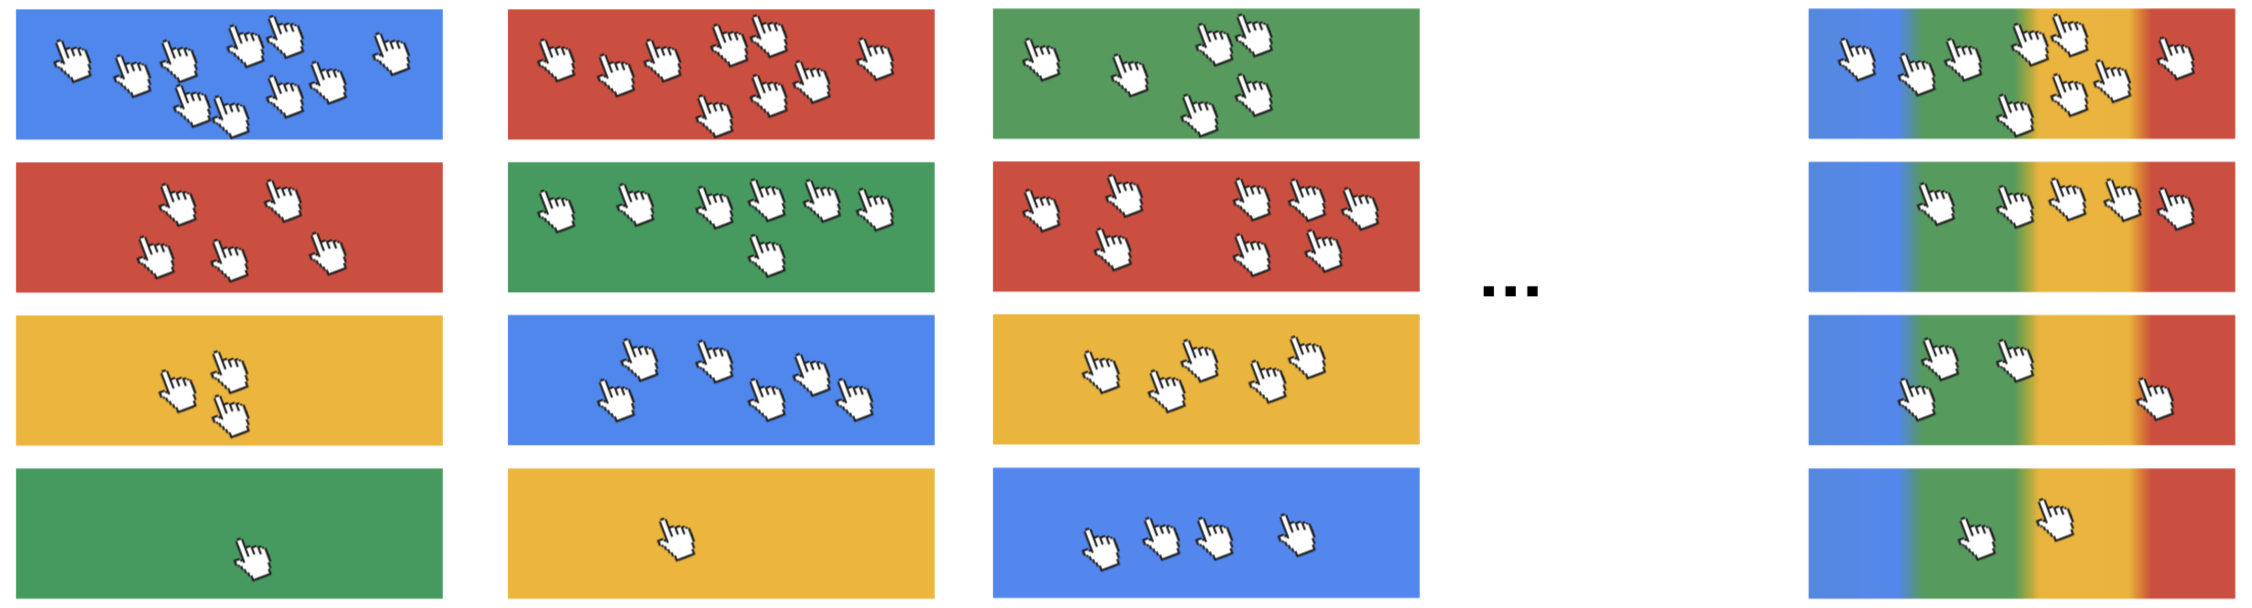
\includegraphics[width=0.8\textwidth]{figures/counterfactual_LTR_RandTopN.png}
			\caption{RandTopN}
		\end{subfigure}
		\begin{subfigure}[b]{0.45\textwidth}
			\centering
			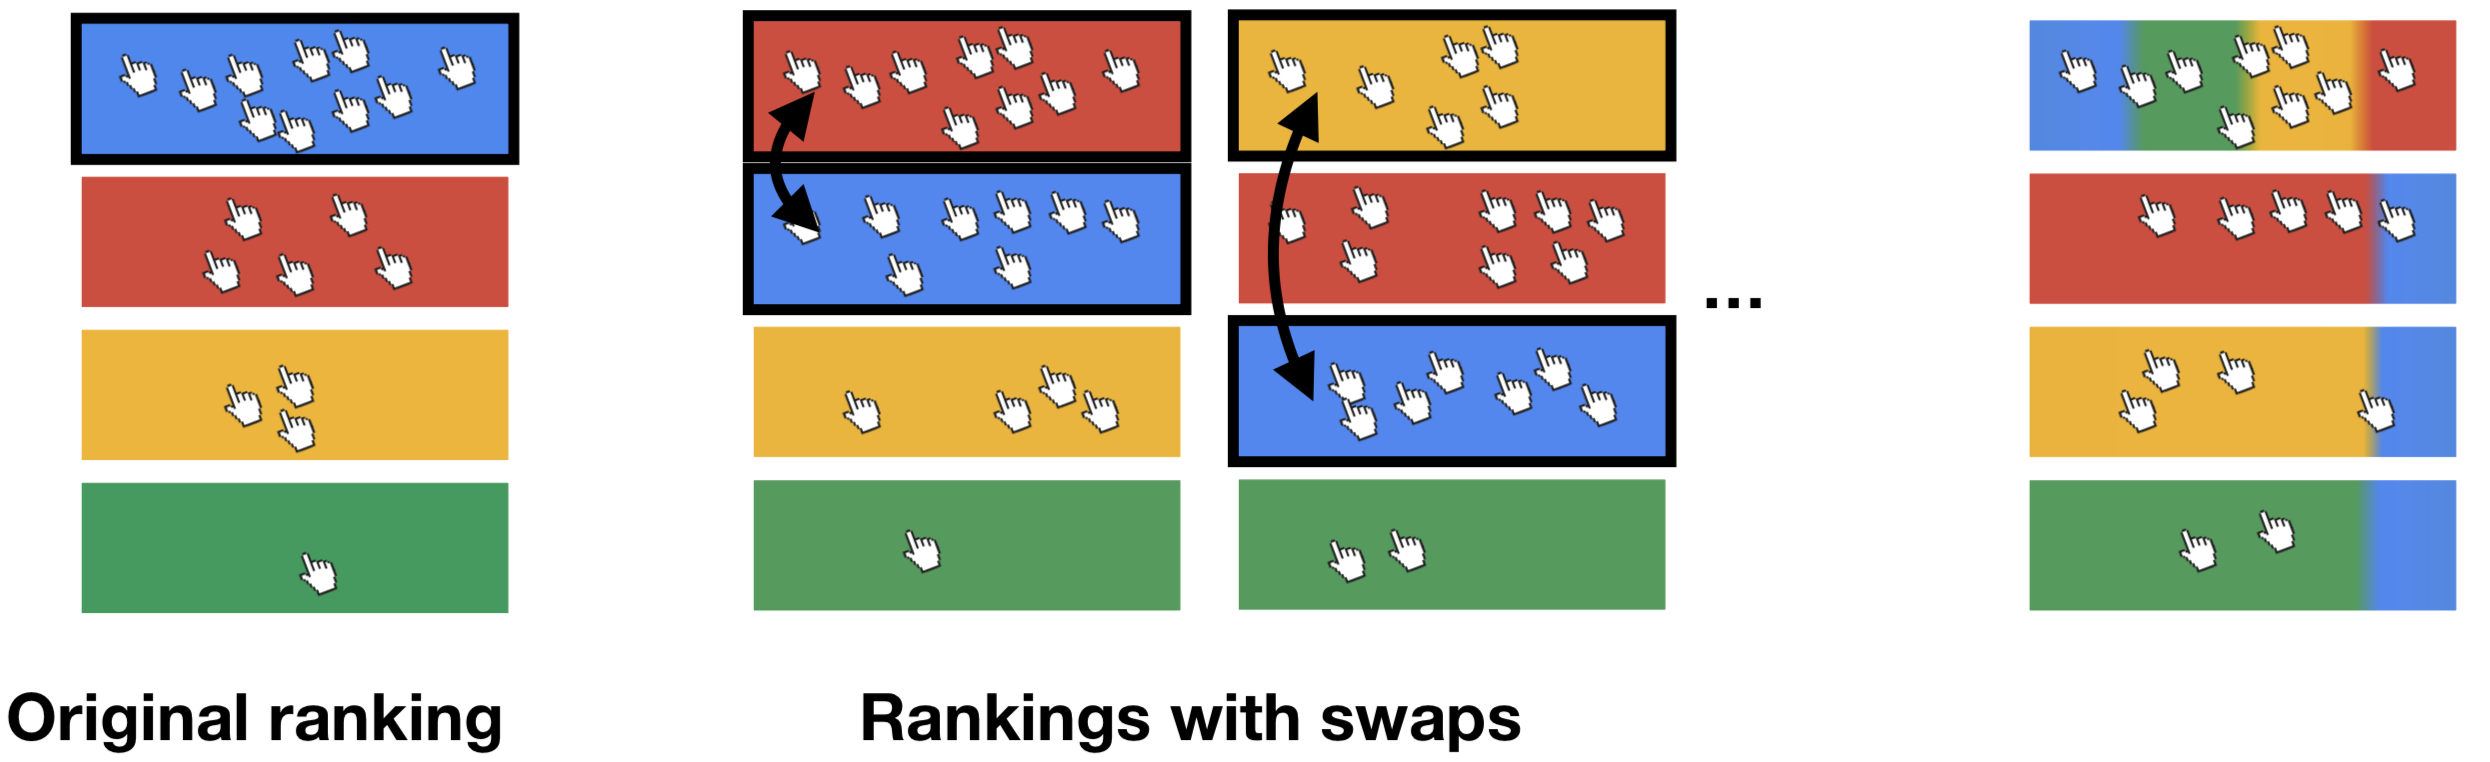
\includegraphics[width=0.8\textwidth]{figures/counterfactual_LTR_RandPair.png}
			\caption{RandPair}
		\end{subfigure}
		\label{img:counterfactual_propensity_estimation}
	\end{figure}
\end{itemize}
\subsubsection{The Variance problem}
\begin{itemize}
	\item The problem of solving the counterfactual approach is that if $p(\textit{observing} \delta_i)$ heads to $0$, the overall objective will be heavily biased towards this example $\implies$ overfitting on single data point
	\item One way to overcome this problem is using a variance regularizer which prevents the policy to deviate too much from the original production policy $\pi_{\text{production}}$:
	$$\pi_{\text{new}} = \arg\min_{\pi} \sum\limits_{i=1}^{N} \frac{\text{rank}\left(\pi(x_i),y_i,\delta_i\right)}{p(\textit{observing }\delta_i)} + \lambda \sqrt{\frac{\mathcal{V}[\pi, \pi_{\text{production}}]}{n}}$$
	\item However, this optimization problem cannot be solved by SGD anymore and iterative methods must be applied (new learning framework \textit{counterfactual risk minimization})
\end{itemize}